\documentclass{article}
\usepackage[margin=1in]{geometry}
\usepackage{mathtools, amsfonts, amsthm, graphicx, listings, xcolor}


\definecolor{codegreen}{rgb}{0,0.6,0}
\definecolor{codegray}{rgb}{0.5,0.5,0.5}
\definecolor{codepurple}{rgb}{0.58,0,0.82}
\definecolor{backcolour}{rgb}{0.95,0.95,0.92}

\lstdefinestyle{mystyle}{
    backgroundcolor=\color{backcolour},   
    commentstyle=\color{codegreen},
    keywordstyle=\color{magenta},
    numberstyle=\tiny\color{codegray},
    stringstyle=\color{codepurple},
    basicstyle=\ttfamily\footnotesize,
    breakatwhitespace=false,         
    breaklines=true,                 
    captionpos=b,                    
    keepspaces=true,                 
    numbers=left,                    
    numbersep=5pt,                  
    showspaces=false,                
    showstringspaces=false,
    showtabs=false,                  
    tabsize=2
}

\lstset{style=mystyle}

\title{Title}
\author{Sam Ly}

\begin{document}
\maketitle

\section*{Part A: By Hand (15 points)}

\textbf{Edges:} \((1,2), (1,3), (2,3), (3,4), (4,5), (4,6), (5,6), (5,7), (6,7), (7,8)\)

\noindent\textbf{Nodes:} \(\{1,2,3,4,5,6,7,8\}\)

\noindent \textbf{No. Edges:} 10

\begin{center}
    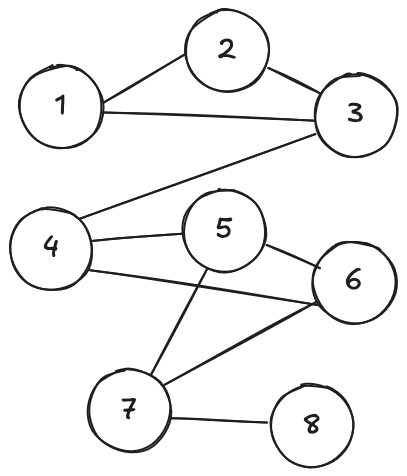
\includegraphics[width=0.3\textwidth]{figures/main_graph.png}
\end{center}

\begin{enumerate}
    \item {
        Density (3 points)
        \begin{itemize}
            \item {
                Write the formula for density.

                \[D = \frac{2E}{N(N-1)}\]
            }

            \item {
                Count nodes and edges.

                8 nodes, 10 edges.
            }

            \item {
                Compute the desnity of this graph.

                \[D = \frac{2(10)}{8(7))} = 0.357\]
            }
        \end{itemize}
    }

    \item {
        Local Clustering Coefficient for Node 3 (3 points)

        \begin{itemize}
            \item {
                Write the formula.

                \[C_i = \frac{2E_i}{k_i(k_i-1)}\]
            }

            \item {
                Identify Node 3’s neighbors.

                Node 3's neighbors are node 1, node 2, and node 4.
            }

            \item {
                Count edges among them.

                There is one edge between node 3's neighbors: \((1,2)\).
            }

            \item {
                Compute \(C_3\).

                \[C_3 = \frac{2(1)}{3(2)} = \frac{1}{3}\]
            }
        \end{itemize}

        \item {
            Global Clustering Coefficient (3 points)

            \begin{itemize}
                \item {
                    Compute the local clustering coefficient for each node with 
                    degree \(\ge\) 2.

                    \begin{center}
                        \begin{tabular}{c c c c}
                            Node \(i\)  & \(k_i\)   & \(E_i\)   & \(C_i\)   \\
                            1           & 2         & 1         & 1         \\
                            2           & 2         & 1         & 1         \\
                            3           & 3         & 1         & \(\frac{1}{3}\)\\
                            4           & 3         & 1         & \(\frac{1}{3}\)\\
                            5           & 3         & 2         & \(\frac{2}{3}\)\\
                            6           & 3         & 2         & \(\frac{2}{3}\)\\
                            7           & 2         & 1         & 1         \\
                            8           & -         & -         & -         \\
                        \end{tabular}
                    \end{center}
                }

                \item {
                    Average them.

                    \[C = \frac{1}{7} \sum_{i=1}^{7}C_i = \frac{1 + 1 + \frac{1}{3} + \frac{1}{3} + \frac{2}{3} + \frac{2}{3} + 1}{7} = \frac{5}{7}\]
                }
                
                
            \end{itemize}

            \item {
                Average Path Length (4 points)

                \begin{itemize}
                    \item {
                        List all unique pairs of nodes.

                        \begin{description}
                            \item[Starting at 1] \((1,2), (1,3), (1,4), (1,5), (1,6), (1,7), (1,8) \)
                            \item[Starting at 2] \((2,3), (2,4), (2,5), (2,6), (2,7), (2,8) \)
                            \item[Starting at 3] \((3,4), (3,5), (3,6), (3,7), (3,8) \)
                            \item[Starting at 4] \((4,5), (4,6), (4,7), (4,8) \)
                            \item[Starting at 5] \((5,6), (5,7), (5,8) \)
                            \item[Starting at 6] \((6,7), (6,8) \)
                            \item[Starting at 7] \((7,8) \)
                        \end{description}
                    }

                    \item {
                        Find the shortest distance \(d(i, j)\) for each pair.

                        \begin{tabular}{c|*{8}{c}}
                                  & 1 & 2 & 3 & 4 & 5 & 6 & 7 & 8 \\ \hline
                                1 &   & 1 & 1 & 2 & 3 & 4 & 4 & 5 \\
                                2 &   &   & 1 & 2 & 3 & 4 & 4 & 5 \\
                                3 &   &   &   & 1 & 2 & 2 & 3 & 4 \\
                                4 &   &   &   &   & 1 & 1 & 2 & 3 \\
                                5 &   &   &   &   &   & 1 & 1 & 2 \\
                                6 &   &   &   &   &   &   & 1 & 2 \\
                                7 &   &   &   &   &   &   &   & 1 \\
                                8 &   &   &   &   &   &   &   &   \\
                        \end{tabular}
                    }

                    \item {
                        Compute the average: 2.36.
                    }
                \end{itemize}
            }

            \item {
                Communities (by eye) (2 points)

                \begin{itemize}
                    \item Groups \{1, 2, 3\} and \{4, 5, 6 ,7, 8\} seem to be communities.
                    \item {
                        Nodes \{1, 2, 3\} form a triangle, while \{4, 5, 6\} 
                        and \{5, 6, 7\} also form triangles.
                    }
                \end{itemize}

            }
        }
    }
\end{enumerate}

\section*{Part B: Coding (10 points)}

\lstinputlisting[language=Python]{./code/main.py}

Outputs from code:
\begin{verbatim}
density 0.35714285714285715
clustering coef 0.3333333333333333
avg. path length 2.2857142857142856
modularity 0.355

\end{verbatim}

\section*{Part C: Reflection (5 points)}

The results from the hand-calculation mostly lined up with the results from the 
code. The only real discrepancy was between the average path length. This is likely
due to the code including the paths starting and ending on the same node in the 
calculation of the average, but my hand calculation doesn't include these paths.
The communities that I indentified by eye matched up decently with those suggested 
by the modularity score. However, I recognize that this technique doesn't scale. 
If this graph was an online community, it would suggest that nodes \{1, 2, 3\} 
form a relatively tight community and is connected to another community \{4, 5, 6, 7, 8\} 
via a single bridge.
\end{document}